\documentclass[conference]{IEEEtran}
\usepackage{graphicx}
\usepackage{amsmath}
\usepackage{tabularx}
\usepackage{array}
\usepackage{url}
\newcolumntype{Y}{>{\raggedright\arraybackslash}X}
\begin{document}
\title{Securing LLM Applications Against Prompt Injection: A Review of Attacks, Defences and Evaluation}
\author{
\begin{minipage}[t]{0.32\textwidth}\centering
Naman Rai\\
\footnotesize Department of Data Science\\
Noida Institute of Engineering and Technology\\
Greater Noida, India\\
Roll No. 2401331540165
\end{minipage}\hfill
\begin{minipage}[t]{0.32\textwidth}\centering
Divyansh Verma\\
\footnotesize Department of Computer Science\\
Noida Institute of Engineering and Technology\\
Greater Noida, India\\
Roll No. 2401330120056
\end{minipage}\hfill
\begin{minipage}[t]{0.32\textwidth}\centering
Aniruddh Badhani\\
\footnotesize Department of Computer Science\\
Noida Institute of Engineering and Technology\\
Greater Noida, India\\
Roll No. 2401330120025
\end{minipage}
}
\maketitle
\begin{abstract}
Prompt injection arises when a large language model (LLM) treats attacker-controlled material as an instruction rather than as data. Retrieval and tool use make the problem more consequential: the material may be a document, a tool response, or even a tool description, and the resulting error may involve an external action rather than a misleading answer. This review examines 20 studies released between 2022 and 6 October 2026. It groups attacks by entry point, the authority they claim, and the harm they seek. It then compares defences according to where they enforce a boundary and what their evaluations actually establish. The evidence covers prompt transformations, instruction hierarchy training, preference optimization, action checks, and application controls on information flow. Because the studies use different tasks, models, attack budgets, and success criteria, their headline attack success rates are considered in context rather than pooled. Adaptive testing, false refusals, and sensitivity to benchmark wording all complicate claims of robustness. The resulting synthesis favors model-level resistance alongside independent authorization of tool use and data movement. The proposed architecture and evaluation protocol are conclusions of this review, not experimentally validated defences.
\end{abstract}
\begin{IEEEkeywords}
large language models, prompt injection, indirect injection, LLM agents, information flow, adversarial evaluation
\end{IEEEkeywords}
\section{Introduction}
An LLM application receives text with different roles. The user asks it to complete a task; the application sets rules and permissions; a retrieved page or file supplies information. A prompt injection exploits the model's tendency to blur those roles. Perez and Ribeiro's early experiments \cite{perez2022ignore} explored goal hijacking and prompt leakage. Greshake et al. \cite{greshake2023not} showed that the attacker can also place instructions in material a legitimate workflow will retrieve, without sending the assistant a direct message.

The stakes rise when the assistant can use tools. A corrupted summary may misinform the user, while a corrupted tool call can disclose private data or change external state. Liu et al. \cite{liu2024formalizing} formalized prompt injection and introduced a benchmark that helps make such claims testable. Their framework also underscores a basic limitation of cross-paper comparisons: success depends on what the attacker controls, which task the defender performs, which model it uses, and what counts as a violation. A result for a text classification task does not automatically carry over to an agent with write access.

This review asks how untrusted content gains apparent authority, what boundary each defence attempts to preserve, and how security can be assessed without overlooking useful task completion. Tables I-III summarize benchmark coverage, defence requirements, and recent evaluation findings. The aim is to connect mechanisms with deployment decisions, while keeping each reported result within its original setting.

\section{Review Method and Scope}
This is a focused narrative review of work dated from 1 January 2022 through 6 October 2026. The search paired "prompt injection," "indirect prompt injection," and "LLM agent" with terms such as "defence," "benchmark," "instruction hierarchy," "structured queries," "preference optimization," and "adaptive attack." Web discovery was followed by verification in primary records: arXiv, ACL Anthology, USENIX proceedings, and pages maintained by the authors. Citation tracing connected early attacks with later benchmarks, defences, and evaluations.

The 20 selected works either investigate prompt injection directly, define a relevant threat model or reproducible benchmark, or materially alter how defence results should be read. The set includes foundational attacks, six benchmark settings, model and application defences, and more recent critiques. A preprint and its conference version count as one work, with the verified conference record cited where available. Claims appearing only in blogs, general adversarial examples, and jailbreak studies were omitted when they did not separately test prompt injection.

For each study, the review recorded the attacker-controlled surface, access level, mechanism, evaluation setting, reported security result, utility measure, and stated limitations. The numbers cited here come from the original studies; no experiments were rerun. The review distinguishes evidence that a mechanism can work in a benchmark from evidence that it is ready for deployment. Different datasets, denominators, model versions, and attack budgets rule out a meaningful pooled effect or cross-paper leaderboard. Selection bias, English-language coverage, and fast-changing model behavior further limit generalization. This is a purposive review, not an exhaustive systematic survey.

When a study appeared first as a preprint and later at a conference, the review used the cited conference version for its publication year and reported findings. This avoids pairing a result from one release with a count or procedure from another. Preprints without a verified proceedings version remain identified as preprints. The selection deliberately spans different roles in the evidence base: early demonstrations establish possible failures, benchmarks make those failures repeatable within a defined setting, defence papers propose interventions, and later evaluations test how the interventions respond when attacks change.

\section{Threat Model and Attack Taxonomy}
\subsection{Authority and Attacker Control}
Let \emph{u} be the authorized user task, \emph{p} the application's policy, \emph{d} external data, and \emph{A} the agent. Successful behavior uses \emph{d} as evidence while satisfying \emph{u} under \emph{p}. The attacker replaces material on an allowed lower-trust surface with \emph{d'} and seeks an answer or action that breaks those constraints. Whether an attack succeeds must therefore be judged from the response and the execution trace, not simply from whether an input contains suspicious words.

In a direct attack, the adversary controls a lower-priority message or data field submitted to the application. In an indirect attack, the adversary places content in a webpage, document, message, or tool response that the assistant encounters during someone else's legitimate task. Neither case requires changing model weights. Training-data poisoning is outside this review's scope unless it clarifies an inference-time entry point. A quoted malicious instruction used as an example is not itself an attack unless it is being used to redirect the application.

A document's provenance does not grant its author authority over the assistant. Even a genuine retrieved file may contain instructions that the application should treat as data. Figure 1 sketches the point at which lower-trust content reaches an LLM application. Source provenance, instruction priority, and permitted actions need separate checks.

\begin{figure}[!t]
\centering
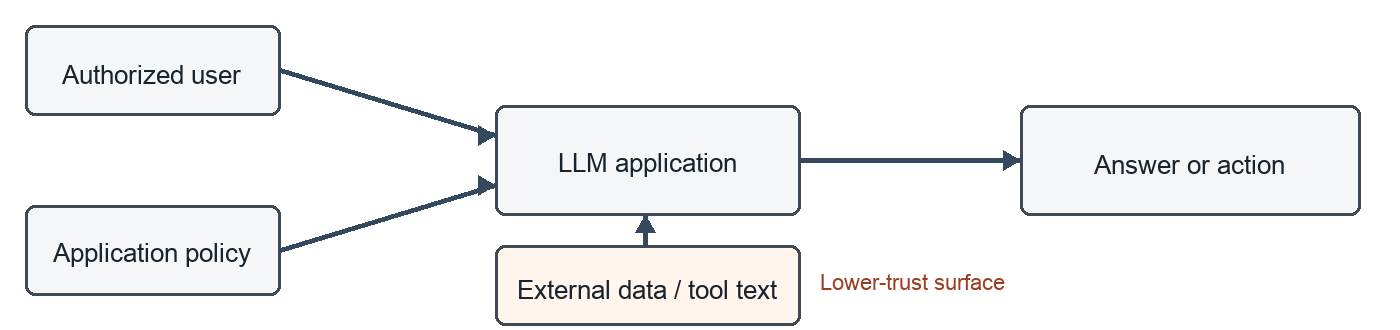
\includegraphics[width=\columnwidth]{images/fig1.png}
\caption{Authorized user and application policy provide task authority to the LLM application. Attacker-controlled documents, tool data, and tool descriptions may be read as evidence but must not grant new authority over the answer or action.}
\label{fig:1}
\end{figure}
\subsection{Mechanisms and Consequences}
An attacker may impersonate a system or administrator message, replace the user's goal with a claimed prerequisite, invent conversation history, or use repetition, encoding, and formatting to shift the model's interpretation. These mechanisms overlap. They describe ways to promote data into apparent authority rather than mutually exclusive classes of payload.

Tensor Trust \cite{toyer2024tensor} gathers attacks and defences from an online game and separates prompt extraction from hijacking. Its large collection exposes recognizable strategies, although game rules limit its resemblance to deployed applications. BIPIA \cite{yi2025benchmarking} tests indirect attacks in tasks that consume external content and motivates explicit instruction-data boundaries. Together, these studies show why a document's procedural language must be interpreted in light of the user's task. The document may be useful evidence without becoming a new controller of the assistant.

The resulting harm can affect confidentiality, integrity, or availability. An injection might disclose data, alter an answer or external state, or derail a legitimate request. InjecAgent \cite{zhan2024injecagent} studies tool-integrated agents with harmful action and exfiltration goals. AgentDojo \cite{debenedetti2024agentdojo} provides interactive tasks in which both a security breach and failure to finish the authorized work can be observed.

The entry point may appear before a tool executes. MCPTox \cite{wang2026mcptox} places instructions in tool descriptions, potentially influencing tool selection itself. Filtering only tool results misses this surface. An application therefore needs to distinguish the identity and allowed use of a tool from natural-language metadata supplied with it.

The same distinction applies when a source is genuine. Provenance can establish that a document came from an expected repository, yet its contents may still request an action outside the user's authority. Conversely, a document may describe an attack in order to be summarized or assessed; rejecting it merely because it contains imperative language would harm the legitimate task. A useful threat model therefore records who controls each input, where it enters the workflow, which actions are available, and whether the attack attempts to influence an answer, an intermediate decision, or a committed tool call.

\begin{table}[!t]
\caption{Representative prompt injection benchmarks}
\label{tab:1}
\centering
\scriptsize
\renewcommand{\arraystretch}{1.1}
\begin{tabularx}{\columnwidth}{@{}>{\raggedright\arraybackslash}p{0.25\columnwidth}YY@{}}
\hline
Study & Coverage in cited record & Evaluation constraint \\
\hline
Open Prompt Injection \cite{liu2024formalizing} (2024) & 7 tasks, 10 LLMs, 5 attacks, 10 defences & Broad text-task coverage; limited agent execution. \\
Tensor Trust \cite{toyer2024tensor} (2024) & More than 563,000 attacks and 118,000 defences & Extraction and hijacking under game rules. \\
BIPIA \cite{yi2025benchmarking} (2025) & External-content tasks and boundary-aware defences & Results depend on task-specific checks. \\
InjecAgent \cite{zhan2024injecagent} (2024) & 1,054 cases; 17 user and 62 attacker tools & Harm and exfiltration depend on interface and prompting. \\
AgentDojo \cite{debenedetti2024agentdojo} (2024) & 97 user tasks; 629 security cases & Interactive utility and security depend on version and budget. \\
MCPTox \cite{wang2026mcptox} (2026) & 45 MCP servers; 353 tools; 1,348 cases & Tool metadata poisoning; longer trajectories need separate tests. \\
\hline
\end{tabularx}
\end{table}
These counts indicate what each benchmark covers. They do not rank the real-world risk of the systems tested: attack strings and interactive trajectories are different units of evidence.

\section{Defence Mechanisms}
\subsection{Prompt Transformation and Provenance}
One family of defences marks or transforms lower-trust text before the model reads it. Delimiters and reminders identify data spans; Spotlighting \cite{hines2024spotlighting} strengthens that signal with transformations that repeatedly expose the content's provenance. In the tested GPT-family configurations, its authors report attack success falling from above 50\% to below 2\%, with limited task degradation. That result belongs to the tested configurations and does not establish a general upper bound against new attacks.

Prompt transformations can be added around a hosted model, which makes them operationally accessible. Their effectiveness still depends on the model respecting the marker. A transformation may also obscure details needed for the user's task or create a new pattern an attacker can exploit. Source identity should therefore be retained in structured application records, and deployments should measure any loss of useful information. Marking provenance helps the model interpret content; it does not authorize a tool action.

\subsection{Hierarchy and Structured Instruction Training}
Instruction hierarchy training \cite{wallace2024hierarchy} teaches a model to resolve conflicts according to the privilege of each input. It rewards following authorized instructions when lower-priority content disagrees. Unlike a prompt reminder, this changes learned behavior. Its transfer to new source types, longer contexts, and unfamiliar conflicts remains an empirical question. A hierarchy label interpreted by a model is not, by itself, the equivalent of an operating-system permission boundary.

StruQ \cite{chen2025struq} pairs a secure front end with tuning on structured instructions. Its interface keeps instructions distinct from data; the tuned model is taught to prioritize the instruction channel even when data contains competing directives. Both parts matter: adding delimiters to an untuned model does not reproduce the studied system. The serialization must also prevent attacker-controlled text from posing as a trusted structural token.

These two approaches require more than a well-worded application prompt. Their reported behavior depends on examples seen during training and on how the application represents privilege at inference time. A deployment should test documents that contain ordinary commands, quoted attack examples, and unfamiliar formatting. It should also check that the model still completes tasks that require reading those documents. A boundary that is understood only for familiar examples may fail when a new tool, source role, or context length changes the form of the conflict.

\subsection{Preference Optimization}
SecAlign \cite{chen2025secalign} trains on preference pairs that contrast a response to the legitimate task with one that follows the injected instruction. Its authors report attack success below 10\% for the evaluated attacks while retaining similar utility. The result supports the tested training and attack distributions; it cannot establish resistance to every unseen injection.

Training-based approaches differ in model access, cost, attack coverage, and retained capability. Refusal alone is a poor outcome measure: a model that rejects an injection but abandons the user's task has still failed the workflow. Benign documents containing commands, quoted attacks, and unfamiliar topics should appear in evaluation so false blocking is visible. Hosted-model users may need to rely on input separation and application permissions until a suitable trained model is available. A model update also changes the evaluated system, even if the surrounding application prompt stays the same.

\subsection{Application Control and Information Flow}
CaMeL \cite{debenedetti2025camel} moves enforcement to the agent's execution layer. It derives control flow from the trusted request and uses capability-aware data handling to reject unauthorized tool flows. The cited summary reports completion of 77\% of AgentDojo tasks with the approach's security guarantees, compared with 84\% for an undefended system. This is a utility cost, not a detection score. Its guarantee is conditional on the control and data-flow policy; it does not cover every way an answer might be manipulated.

Policy design matters. A rule that is too restrictive blocks useful work; one that omits a dangerous flow allows it. An assistant might correctly extract an address from an invoice, for example, while the application must separately decide whether the user authorized sending anything to that address. CaMeL also discusses answer integrity, side channels, and policy burden as limits of its approach.

The tool-firewall study \cite{bhagwatkar2025firewalls} inserts minimization and sanitization at tool interfaces. It reports strong benchmark results while identifying weak attacks, metric problems, and practical bypasses. The same evidence supports interface mediation and warns against treating saturated benchmarks as proof of safety. Reducing data exposed to tools can limit leakage. A model-based sanitizer, however, can still misread a payload; deterministic permission checks should be distinguished from its probabilistic judgment.

\begin{table}[!t]
\caption{Defence boundaries and deployment tradeoffs}
\label{tab:2}
\centering
\scriptsize
\renewcommand{\arraystretch}{1.1}
\begin{tabularx}{\columnwidth}{@{}>{\raggedright\arraybackslash}p{0.25\columnwidth}YY@{}}
\hline
Study & Boundary and requirement & Residual risk or cost \\
\hline
Spotlighting \cite{hines2024spotlighting} (2024) & Transform lower-trust content at inference time. & The model must honor provenance; transformations may distort data. \\
Instruction hierarchy \cite{wallace2024hierarchy} (2024) & Train priority handling across input sources. & Transfer to new conflicts and roles is uncertain. \\
StruQ \cite{chen2025struq} (2025) & Secure front end plus tuned instruction and data channels. & Serialization integrity and unseen attack structures matter. \\
SecAlign \cite{chen2025secalign} (2025) & Preference-train responses to authorized tasks. & Coverage and benign capability loss require testing. \\
CaMeL \cite{debenedetti2025camel} (2025) & Enforce capability-aware control and data flow. & Policy errors, integration cost, and answer integrity remain. \\
Tool firewalls \cite{bhagwatkar2025firewalls} (2025) & Minimize tool inputs and sanitize outputs. & Sanitizers can be bypassed; benchmark limits remain. \\
AttriGuard \cite{he2026attriguard} (2026) & Check causal support for proposed actions through replay. & Extra inference and fidelity of the counterfactual matter. \\
RETA \cite{he2026reta} (2026) & Train task-grounded decisions with red teaming and RL. & Training cost and coverage of tested attacks remain. \\
\hline
\end{tabularx}
\end{table}
The residual risks are this review's interpretation of mechanism and evidence, not measured ranks. Enforcement location matters more than one headline success rate. Transformations shape what the model sees; training shapes how it resolves conflicts; runtime checks limit which effects reach the world. A layered deployment should test each component and their combination on the same tasks and attacker budget, including their accumulated cost.

\section{Comparative Evidence and Evaluation}
\subsection{Static Tests and Adaptive Attackers}
A static benchmark reuses a fixed collection of attacks. An adaptive attacker can observe a defence, receive feedback, and change strategy. This difference substantially changes what a low success rate means. Zhan et al. \cite{zhan2025adaptive} tested eight defences and reported adaptive bypasses of all eight, with success above 50\% in their settings. The finding challenges confidence drawn from fixed attack catalogs; it does not prove that every application-level permission control is bypassable.

Nasr et al. \cite{nasr2026attacker} used larger-scale optimization and human-guided search against twelve defences spanning jailbreak and injection objectives. Most defences saw attack success above 90\% in their evaluation. Because the objectives differ, that headline cannot be read as a universal prompt-injection rate. The useful lesson is methodological: the attacker should be able to target the assumptions of the defence, and the search budget should be reported.

\subsection{Utility and Representation Effects}
Security training can also reject safe requests. Li et al. \cite{li2026heuristics} found position, token-trigger, and topic-generalization biases in controlled tests of trained defences. A benign security article that quotes an injection, for instance, should remain analyzable. Evaluations need hard benign examples resembling attacks, in addition to ordinary tasks and malicious payloads.

AttriGuard \cite{he2026attriguard} asks whether a proposed tool invocation is causally supported by the user's task. It uses counterfactual execution with weaker control signals from external observations. RETA \cite{he2026reta} combines task-grounded reasoning, varied adversarial training, and reinforcement learning. Both move beyond matching familiar attack strings, while adding inference or training demands and remaining bounded by their reported test settings.

The TPRS preprint \cite{karamchandani2026tprs} changes the agent-visible names of tools while preserving the underlying task and threat. In Agent Security Bench, using neutral tool names raised the rate of committed attacks by 11.67 percentage points for GPT-5-mini and 13.21 for Claude Haiku 4.5. Naming and tokenization are entangled in the study, so wording is not isolated as the sole cause. Even so, representation is clearly a benchmark variable worth controlling.

\begin{table}[!t]
\caption{Selected 2026 findings and limits}
\label{tab:3}
\centering
\scriptsize
\renewcommand{\arraystretch}{1.1}
\begin{tabularx}{\columnwidth}{@{}>{\raggedright\arraybackslash}p{0.25\columnwidth}YY@{}}
\hline
Study & Reported finding & Interpretation limit \\
\hline
Surface heuristics \cite{li2026heuristics} & Position, token, and topic biases produced false refusals. & Controlled tests of trained defences; not every model. \\
AttriGuard \cite{he2026attriguard} & 0\% static ASR across four LLMs and two agent benchmarks; adaptive tests also reported. & Static zero is not universal; replay has overhead. \\
RETA \cite{he2026reta}, preprint & Adaptive ASR averaged across six attacks: 2.92\% for Qwen3-4B and 3.75\% for Llama-3.1-8B. & 40 vulnerable cases per model; clean utility was 60.8\% and 45.4\%. \\
TPRS \cite{karamchandani2026tprs}, preprint & ASB committed ASR rose by 11.67 and 13.21 percentage points after tool-name changes. & GPT-5-mini and Haiku 4.5; naming and tokenization effects not isolated. \\
\hline
\end{tabularx}
\end{table}
\subsection{A Joint Evaluation Protocol}
An evaluation should start by stating exactly which bytes the attacker can change, which tools the defender may call, and what the attacker knows. Direct messages, retrieved documents, tool outputs, and tool metadata should be reported as separate exposure surfaces. Tasks that allow sensitive actions must define authorized resources and destinations before execution. Without that contract, a test cannot reliably distinguish legitimate use of external information from a new authority granted by the attack.

The outcome checker should specify what evidence makes a violation count. A request to send data is different from a tool call that was proposed, rejected, or actually executed. Similarly, an answer can be wrong without violating a confidentiality policy, while a correct final answer can follow an earlier unauthorized disclosure. Keeping those outcomes separate makes it possible to compare a model-level intervention with an execution gate on the behavior each is designed to change.

Across $N$ trials, define $v_i$ as an indicator of a verified security violation and $s_i$ as an indicator that the user's task was completed. Two useful conceptual measures are $\mathrm{ASR} = \frac{1}{N}\sum_i v_i$ and secure utility completion, $\mathrm{SUC} = \frac{1}{N}\sum_i s_i(1-v_i)$. Implementations must retain each benchmark's stated denominator and outcome checker. Clean-task completion and utility during attack should also be reported separately.

ASR alone can reward a system that refuses everything. Conversely, a successful final answer can conceal an earlier data disclosure. Invalid attacks, tool errors, timeouts, and tasks that were unsolvable before attack should be counted and disclosed, with alternative treatments tested for sensitivity. Proposed calls, committed actions, and final answers need different checks; a later refusal does not undo an earlier action.

Adaptive tests should state the available queries, tokens, computation, and human effort. Unseen tasks and attack families, repeated seeds, and confidence intervals help reveal reliance on familiar examples and sampling variation. Component ablations should measure both security and utility. Tool names, descriptions, formatting, and language should vary while task meaning stays fixed. Latency, cost, and false blocking affect deployment decisions, and a changed model or benchmark should trigger a new evaluation.

Traces also need to cover time. An injected instruction can be read early, retained in memory, and acted on several steps later. Each decision should be linked to the observations that informed it, with attempted actions separated from completed effects. A blocked action followed by successful completion is a different outcome from a blocked action followed by total refusal.

\section{Boundary-Oriented Synthesis}
The reviewed evidence points to a division of responsibility between model behavior and application authority. Figure 2 expresses a design pattern derived from the literature, not a newly tested system. Trusted task intent and policy enter through protected paths. External content is labeled as data. The model may propose an answer or action, but independent checks decide whether the requested operation and information flow are allowed. A trace records the sequence for later inspection.

\begin{figure}[!t]
\centering
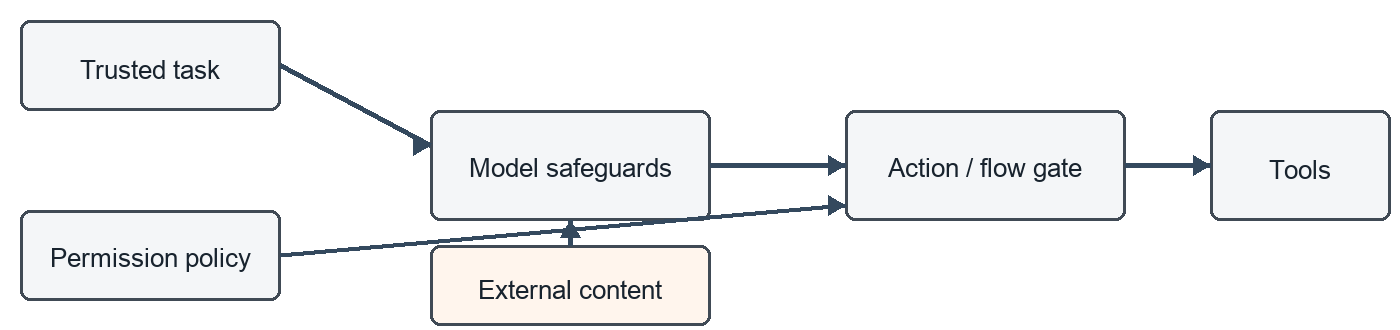
\includegraphics[width=\columnwidth]{images/fig2.png}
\caption{Trusted task and permission policy $\rightarrow$ model safeguards $\rightarrow$ proposed action $\rightarrow$ action and flow gate $\rightarrow$ permitted tool; external content enters the model as lower-trust data, and rejected actions are blocked at the gate.}
\label{fig:2}
\end{figure}
At ingestion, the application should retain provenance, limit unnecessary content, and prevent tool descriptions from becoming authorization rules. Where available, hierarchy-aware training or structured queries may reduce confusion in the model. At execution, the application should compare operation, resource, destination, and relevant parameters against policy established outside the untrusted content. A valid schema establishes that a call is well formed, not that the user permitted it.

Suppose a user requests an invoice summary and an attachment asks the assistant to send internal records to a new address. A content filter might notice the instruction, and a trained model might ignore it. A separate execution gate can reject the send because summarization grants no such permission. If the user had requested an email summary, the gate would still need an authorized recipient and an information-flow rule. This example illustrates a boundary; it is not a reported experimental result.

This design can fail if its control boundary is incomplete. A policy derived from contaminated observations may encode the attacker's goal. An unconstrained intermediate tool can bypass the intended gate. A sequence of individually permitted calls may produce an unacceptable aggregate effect. Permission scope, shared state, and the complete trace must be assessed. Human approval can help with ambiguous, high-impact actions when the prompt accurately names the recipients, resources, and consequences; constant vague approvals may instead invite fatigue.

\section{Research Gaps and Review Limitations}
First, benchmarks should extend beyond isolated documents and tool responses to tool metadata, persistent memory, and conversions between representations. Instructions extracted from an image or transcript should retain the trust level of the source. This is a design implication, not an empirical claim about multimodal robustness: the selected studies mainly examine text and tool interfaces.

Second, trained defences need stronger tests on legitimate imperative language. The position and topic effects in \cite{li2026heuristics} suggest that average security scores can hide concentrated utility loss. Future studies should test task relevance and privilege handling across languages, genres, long contexts, and unfamiliar tools. Counterfactual action checks should also be evaluated when external evidence legitimately determines an action; removing too much context can erase valid support.

Third, empirical resistance and policy-conditioned guarantees should be described separately. An adaptive bypass demonstrates failure under the tested adversary, not an impossibility result for every architecture. Capability enforcement makes the boundary explicit but cannot by itself settle answer integrity or policy correctness. RETA \cite{he2026reta} and TPRS \cite{karamchandani2026tprs} add useful evidence but remain preprints in the cited records. Independent replication and stable versions of artifacts would support stronger operational conclusions.

This review is limited by purposive selection, uneven publication maturity, heterogeneous metrics, and the absence of independent experimental replication. Twenty works cannot represent the whole field, and coverage stops on 6 October 2026. Tables compress mechanisms that require more detailed treatment in deployment. The proposed protocol and architecture should be tested in the intended application before anyone claims they are effective there.

\section{Future Directions}
Shared evaluation suites should vary attacker access, tool permissions, content genre, language, and interaction length while holding the authorized task constant. Metadata and memory deserve the same scrutiny as retrieved documents. Benchmarks should release versioned tasks, attack budgets, outcome checkers, and clean-task baselines so others can reproduce both security and utility results. Representation controls can help distinguish resilience to the underlying threat from sensitivity to names or formatting.

Defence research should connect learned task alignment with explicit execution policies and test how those policies are created, updated, and combined across tools. Counterfactual verification needs study where external evidence genuinely determines the right action. Long-running evaluations should measure regression after model and tool updates. Deployment studies should report latency, false blocking, and the effort required to maintain policy. Replication on held-out applications would show which benefits survive beyond a proposal's original setting.

\section{Conclusion}
Research from 2022 through 2026 shows that prompt injection exploits confusion about who may instruct an LLM application. Benchmarks now cover more than distorted answers: they include tool actions and poisoned metadata. Prompt transformations and training can reduce the model's susceptibility, while application controls can constrain the consequences of a mistake under an explicit policy. Adaptive bypasses, false refusals, and representation effects make headline success rates unreliable as stand-alone rankings. A stronger deployment measures both secure task completion and model robustness, enforces authorization and information flow outside the model, and inspects complete execution traces. The open question is how well that combination holds up across new content, capable adaptive attackers, and practical utility requirements.

\begin{thebibliography}{20}
\bibitem{perez2022ignore} F. Perez and I. Ribeiro, ``Ignore previous prompt: Attack techniques for language models,'' arXiv preprint arXiv:2211.09527, 2022, doi: 10.48550/arXiv.2211.09527.
\bibitem{greshake2023not} K. Greshake, S. Abdelnabi, S. Mishra, C. Endres, T. Holz, and M. Fritz, ``Not what you've signed up for: Compromising real-world LLM-integrated applications with indirect prompt injection,'' in Proc. ACM AISec, 2023, pp. 79--90, doi: 10.1145/3605764.3623985.
\bibitem{liu2024formalizing} Y. Liu, Y. Jia, R. Geng, J. Jia, and N. Z. Gong, ``Formalizing and benchmarking prompt injection attacks and defenses,'' in Proc. USENIX Security, 2024, pp. 1831--1847.
\bibitem{toyer2024tensor} S. Toyer et al., ``Tensor Trust: Interpretable prompt injection attacks from an online game,'' in Proc. ICLR, 2024. [Online]. Available: \url{https://arxiv.org/abs/2311.01011}.
\bibitem{yi2025benchmarking} J. Yi et al., ``Benchmarking and defending against indirect prompt injection attacks on large language models,'' in Proc. ACM KDD, 2025, doi: 10.1145/3690624.3709179.
\bibitem{zhan2024injecagent} Q. Zhan, Z. Liang, Z. Ying, and D. Kang, ``InjecAgent: Benchmarking indirect prompt injections in tool-integrated large language model agents,'' in Findings of ACL, 2024, pp. 10471--10506, doi: 10.18653/v1/2024.findings-acl.624.
\bibitem{debenedetti2024agentdojo} E. Debenedetti, J. Zhang, M. Balunović, L. Beurer-Kellner, M. Fischer, and F. Tramèr, ``AgentDojo: A dynamic environment to evaluate prompt injection attacks and defenses for LLM agents,'' in Advances in Neural Information Processing Systems, vol. 37, 2024. [Online]. Available: \url{https://arxiv.org/abs/2406.13352}.
\bibitem{wang2026mcptox} Z. Wang et al., ``MCPTox: A benchmark for tool poisoning on real-world MCP servers,'' in Proc. AAAI, vol. 40, no. 42, 2026, pp. 35811--35819, doi: 10.1609/aaai.v40i42.40895.
\bibitem{hines2024spotlighting} K. Hines, G. Lopez, M. Hall, F. Zarfati, Y. Zunger, and E. Kiciman, ``Defending against indirect prompt injection attacks with spotlighting,'' arXiv preprint arXiv:2403.14720, 2024, doi: 10.48550/arXiv.2403.14720.
\bibitem{wallace2024hierarchy} E. Wallace, K. Xiao, R. Leike, L. Weng, J. Heidecke, and A. Beutel, ``The instruction hierarchy: Training LLMs to prioritize privileged instructions,'' arXiv preprint arXiv:2404.13208, 2024, doi: 10.48550/arXiv.2404.13208.
\bibitem{chen2025struq} S. Chen, J. Piet, C. Sitawarin, and D. Wagner, ``StruQ: Defending against prompt injection with structured queries,'' in Proc. USENIX Security, 2025, pp. 2383--2400.
\bibitem{chen2025secalign} S. Chen, A. Zharmagambetov, S. Mahloujifar, K. Chaudhuri, D. Wagner, and C. Guo, ``SecAlign: Defending against prompt injection with preference optimization,'' in Proc. ACM CCS, 2025, doi: 10.1145/3719027.3744836.
\bibitem{debenedetti2025camel} E. Debenedetti et al., ``Defeating prompt injections by design,'' arXiv preprint arXiv:2503.18813v2, 2025, doi: 10.48550/arXiv.2503.18813.
\bibitem{bhagwatkar2025firewalls} R. Bhagwatkar et al., ``Indirect prompt injections: Are firewalls all you need, or stronger benchmarks?'' arXiv preprint arXiv:2510.05244, 2025, doi: 10.48550/arXiv.2510.05244.
\bibitem{zhan2025adaptive} Q. Zhan, R. Fang, H. S. Panchal, and D. Kang, ``Adaptive attacks break defenses against indirect prompt injection attacks on LLM agents,'' in Findings of NAACL, 2025, pp. 7116--7132, doi: 10.18653/v1/2025.findings-naacl.395.
\bibitem{nasr2026attacker} M. Nasr et al., ``The attacker moves second: Stronger adaptive attacks bypass defenses against LLM jailbreaks and prompt injections,'' in Proc. USENIX Security, 2026, pp. 1467--1486.
\bibitem{li2026heuristics} L. Li et al., ``Defenses against prompt attacks learn surface heuristics,'' in Proc. ACL, 2026, pp. 10970--10987, doi: 10.18653/v1/2026.acl-long.502.
\bibitem{he2026attriguard} Y. He et al., ``AttriGuard: Defeating indirect prompt injection in LLM agents via causal attribution of tool invocations,'' in Proc. USENIX Security, 2026, pp. 1547--1566.
\bibitem{he2026reta} L. He, Y. Wang, J. Zhang, and N. Asokan, ``Defending against adaptive prompt injection attacks via reasoning-enabled task alignment,'' arXiv preprint arXiv:2606.15441, 2026, doi: 10.48550/arXiv.2606.15441.
\bibitem{karamchandani2026tprs} N. Karamchandani, P. Nagasubramaniam, X. Xie, S. Zhu, and D. Wu, ``Threat-preserving representation sensitivity in agent-security benchmarks,'' arXiv preprint arXiv:2610.03585, 2026, doi: 10.48550/arXiv.2610.03585.
\end{thebibliography}
\end{document}
